%%% File encoding: UTF-8 äöüÄÖÜß  <-- no German umlauts here? Use an UTF-8 compatible editor!

%%% Magic comments for setting the correct parameters in compatible IDEs
% !TeX encoding = utf8
% !TeX program = pdflatex 
% !TeX spellcheck = de_DE
% !BIB program = biber

\documentclass[bachelor,english,smartquotes]{hgbthesis}

% Valid options in [..]: 
%    Type of work: 'diploma', 'master' (default), 'bachelor', 'internship' 
%    Main language: 'german' (default), 'english'
%    Turn on smart quote handling: 'smartquotes'
%    APA bibliography style: 'apa'
%%%-----------------------------------------------------------------------------

\RequirePackage[utf8]{inputenc} % Remove when using lualatex or xelatex!


% Custom imported packages
\usepackage[bottom]{footmisc}
\usepackage{fancyvrb}
\usepackage{pgf-umlsd}

\graphicspath{{images/}}  % Location of images and graphics
\logofile{logo}           % Logo file: images/logo.pdf (no logo: \logofile{})
\bibliography{references} % Biblatex bibliography file (references.bib)

\definecolor{darkgreen}{rgb}{0.0, 0.5, 0.0}

%%%-----------------------------------------------------------------------------
% Title page entries
%%%-----------------------------------------------------------------------------

\title{Service-to-service Authentication in a Microservice Deployment}
\author{Benjamin Ellmer}
\programname{Mobile Computing}

\programtype{Fachhochschul-Bachelorstudiengang} % select/edit
% \programtype{Fachhochschul-Masterstudiengang}

\placeofstudy{Hagenberg}
\dateofsubmission{2022}{03}{28} % {YYYY}{MM}{DD}

\advisor{FH-Prof. DI Dr. Marc Kurz} % optional

%\strictlicense % restrictive license instead of Creative Commons (discouraged!)

%%%-----------------------------------------------------------------------------
\begin{document}
%%%-----------------------------------------------------------------------------

%%%-----------------------------------------------------------------------------
\frontmatter                                   % Front part (roman page numbers)
%%%-----------------------------------------------------------------------------

\maketitle
\tableofcontents
%\chapter{Preface}






 % A preface is optional
\chapter{Abstract}
The microservice architecture is a currently emerging pattern in software engineering.
Instead of having one huge application, the logic is split into numerous smaller units that fulfill one single purpose.
Therefore function calls within the application migrate to remote calls over the network.
The remote calls between the services have to provide confidentiality, integrity, and authentication.
The Transport Layer Security (TLS) protocol provides confidentiality integrity and authenticates the server to the client, but not the client to the server.
Therefore additional mechanisms are necessary for the mutual authentication of the services.

The most popular service-to-service authentication mechanisms are self-signed JSON Web Tokens (JWT) and mutual TLS (mTLS).
Mutual TLS is an adaptation of the TLS protocol that provides a simple and efficient implementation of service-to-service authentication.
On the other hand, it has few configuration possibilities making it hard to adapt the mechanisms for purposes other than service-to-service authentication.
Self-signed JWTs provide the possibility to embed additional parameters within the JWTs, allowing to adapt the authentication mechanisms to simplify tasks like sharing the end-user context.
Additionally, self-signed JWTs have the significant advantage over mTLS that they allow achieving nonrepudiation by storing the received JWTs and requests.

In the end, it is not valid to say that one authentication mechanism is superior in each situation.
Self-signed JWTs are the preferred authentication mechanism when nonrepudiation is required or when the application shares the end-user context.
mTLS is the preferred authentication mechanism when the aim is to implement service-to-service authentication as simply as possible.
Nevertheless, this does not mean that mTLS is must not be used for complex applications or that self-signed JWTs are inappropriate for simple applications.
		
\chapter{Kurzfassung}

\begin{german}
An dieser Stelle steht eine Zusammenfassung der Arbeit, Umfang
max.\ 1 Seite. 
...
\end{german}			

%%%-----------------------------------------------------------------------------
\mainmatter                                    % Main part (arabic page numbers)
%%%-----------------------------------------------------------------------------

\chapter{Introduction}
\label{cha:Introduction}
In the past years, a trend towards highly-scalable software systems like the microservice architecture emerged.
The migration from a monolithic architecture towards microservices has enormous consequences regarding the security of software systems~\cite{shmeleva2020microservices}. 
Function calls within the same project migrate to remote calls over the network~\cite{chandramouli2019microservices}. 
%TODO: Unclear antecedent
This offers a larger attack surface because intruders could spoof the communication among the services.
Therefore the communication among the services has to provide mutual authentication to prevent attackers from exploiting the system.
Additionally, service-to-service communication has to provide confidentiality.
Confidentiality is usually addressed using TLS, which also provides authentication, but it only authenticates the server to the client.
Therefore additional authentication mechanisms are necessary to implement mutual authentication.
The most popular approaches for service-to-service authentication are mutual TLS (mTLS) and authentication using self-signed JSON Web Tokens (JWT)~\cite{dias2020microservices}.
This thesis will describe and compare those authentication mechanisms to discover differences, advantages, and disadvantages.

\section{Motivation}
The International Data Corporation (IDC) has predicted that by 2022, 90\% of all apps will feature microservice architectures~\cite{idcprediction2019}. 
So it is inevitable to deal with the numerous mechanisms to secure such systems properly. 
Authentication is one of the most crucial security challenges.
When authentication is neglected, attackers could perform attacks like the Main-in-the-middle-Attack to exploit the system, even if other security challenges like confidentiality and integrity are mastered.
Such attacks could result in substantial data leaks or allow attackers to misuse the system for their advantage.

The microservice architecture is based on having multiple services running in multiple locations.
%TODO: Unclear antecedent
This results in a bigger attack surface because multiple machines are exposed to the internet, making it simpler to find vulnerabilities.
%TODO: Unclear antecedent
This is one of the reasons why Netflix received massive attacks on their microservice based-systems in the past years~\cite{pereira2019security}.

These motivations show how vital microservice security is, and this thesis aims to help microservice developers choose the correct authentication mechanisms for their projects.

\section{Challenges}
Since the microservice architecture became as popular as in the last years, there is a lack of evaluation research and only limited insight into the particular security concerns, especially regarding service-to-service authentication. 
The most popular solutions and existing implementations are closed source, like the mTLS Architecture of Netflix.
Other freely available approaches are often poorly documented and therefore hard to understand~\cite{yarygina2018overcoming}.

Additionally, the migration from the monolithic architecture to the microservice architecture results in a performance overhead~\cite{ueda2016workload}.
Furthermore, the authentication mechanisms produce latencies because additional operations have to be performed.
Therefore it is crucial to choose the correct authentication mechanism and implement it as efficiently as possible.

The microservice architecture and the service-to-service authentication bring some more challenges and difficulties, which will be declared and discussed in the following chapters.

\section{Chapter Overview}
Chapter~\ref{cha:Microservice_Architecture} introduces essential fundamentals of the microservice architecture. 
It should explain why the later discussed authentication mechanisms are a requirement caused by the microservice architecture.

\noindent Chapter~\ref{cha:Related_Work} summarizes the state-of-the-art concepts regarding microservice security and public key-based authentication.
Furthermore, it describes the fundamentals of the required technologies for the later discussed authentication mechanisms.

\noindent Chapter~\ref{cha:authentication_mechanisms} describes the fundamentals and concepts of the compared authentication mechanisms in detail.
Especially the motivations, challenges, and differences between them are analyzed.

\noindent Chapter~\ref{cha:project_structure} shows the backend of an app, which implements the discussed authentication mechanisms.
Additionally, it provides some implementation details for the ASP.Net framework.

\noindent Chapter~\ref{cha:experiment} describes the setup of a performance experiment comparing the discussed authentication mechanisms.
The experimental results are then interpreted and discussed.

\chapter{Microservice Architecture}
\label{cha:Microservice_Architecture}
This chapter introduces the microservice architecture concepts necessary to understand why the later discussed approaches are needed.
The principles used to design microservices lead to some characteristics, resulting in the motivations and challenges declared in this chapter.
Furthermore, some recommendations about the use cases of the microservice architecture are provided, and the caused security consequences are declared.

\section{Motivation}
Companies like Netflix, Amazon, and Uber are front-runners for building software solutions using the microservice architecture~\cite{dias2020microservices}.
The main idea is to split the business logic of an application into small autonomous services that work together.
% TODO: Unclear antecedent
This means the programmers have to avoid the temptation of developing too large systems, resulting in the following benefits~\cite{newman2021building}:
\begin{itemize}
    \item Technology heterogeneity is achieved through the possibility to use different technology stacks for different services, depending on the needs of the services.
		It is even possible to use different data storages for the different microservices (e.g., graph database for users).
    \item Resilience is achieved since component failures can be isolated, so the rest of the system can carry on working by degrading the functionality of the system. 
    \item Scaling is much more effective due to the possibility to scale only the parts of the system that really need scaling.
    \item The deployment process is much more convenient because a single microservice can be deployed instead of deploying the whole application, even for small changes.
    \item The organizational alignment can be improved by assigning the work to small teams that work on smaller codebases, resulting in higher productivity.
    \item Composability is achieved, considering that the functionalities can be consumed in different ways for different purposes.
    \item Replaceability is optimized since rewriting a tiny service is much more manageable than replacing a few parts of a vast application.
\end{itemize}

\section{Comparison to the Monolithic Architecture}
\begin{figure}
    \centering
    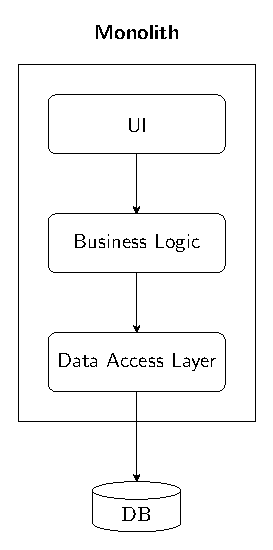
\includegraphics[width=0.3\textwidth]{./images/microservice_architecture/TikZ_Monolith.pdf}
    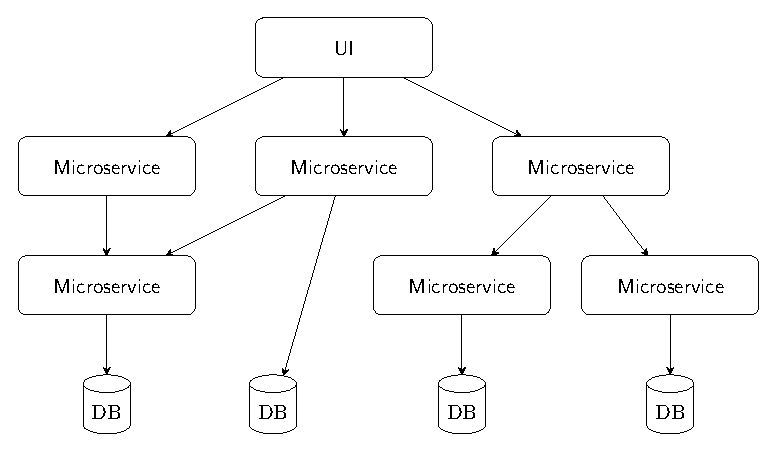
\includegraphics[width=0.69\textwidth]{./images/microservice_architecture/TikZ_Microservice.pdf}
    \caption{Example of monolithic architecture and a microservice architecture~\cite{kalske2017challenges}}
    \label{fig:monolithvsmicroservice}
\end{figure}

Figure~\ref{fig:monolithvsmicroservice} shows the architectural differences between monolithic and microservice applications.
A monolithic application has a single unit containing the user interface layer (UI), the business logic layer, and the data access layer.
Therefore it is much simpler to manage but brings the following downsides regarding the codebase~\cite{kalske2017challenges}:
\begin{itemize}
    \item New features and modifications of old features are harder to implement.
    \item Refactoring changes can reflect many parts of the software.
    \item Code duplication raises since it is almost impossible to reuse existing code.
\end{itemize}
The microservice architecture consists of multiple services focused on only one function of the business logic.
Those services communicate with other services using remote calls (e.g., over HTTP), which causes higher latencies.
Depending on the needs of the services, each service can have its own database, which can differ from the database system of the other services.
It is also possible to share one database for multiple services, but this should be avoided to reduce coupling. 

\section{Design Principles}
It is hard to define principles, which will apply to all microservice architectures, but according to Newman, most of them will adhere to the following principles~\cite{newman2021building}: 
\begin{description}
    \item[Modelled around business concepts:] The functionalities are structured around the business contexts instead of the technical concepts.
    \item[Adopting culture of automation:] The microservice deployments embrace the culture of automation by using automated tests, continuous delivery, automated servers, and much more automation tools.
    \item[Hiding implementation details:] The microservices hide as many implementation details as possible to avoid coupling.
		Especially the databases of the services should be hidden and can be accessed by other services using the APIs of the services.
    \item[Decentralising all the things:] All approaches that could centralize business logic are avoided to keep associated data and logic within the service boundaries.
    \item[Independently deployed:] The microservices should provide the possibility to deploy them without having to deploy any other service.
		Therefore the autonomy of the teams can be increased, and new features can be released faster.
    \item[Isolates failures:] The microservices have to deal with misbehaving parts of the system and keep on providing as much functionality as possible, to prevent cascading failure.
    \item[Highly observable:] It is not sufficient to observe a single service's behavior and status.
		Instead, the functioning of the whole system has to be monitored.
\end{description}

\section{Challenges} \label{sec:microservice_challenges}
The microservice architecture brings numerous benefits, but it also introduces a set of challenges, which could argue to avoid the microservice architecture in some cases.
According to Kalske et al.~\cite{kalske2017challenges} the microservice architecture brings the following technical challenges with it: 
\begin{itemize}
    \item The declaration of the service boundaries is very hard~\cite{kalske2017challenges}, especially if the developers do not know the domain very well~\cite{newman2021building}.
    \item The services should not become too fine-grained to prevent performance overhead.
		Otherwise, if they are not decomposed enough, one service can affect multiple services.
    \item Continuous Delivery and Continuous Integration are necessary to manage the services and validate their functionality.
    \item The integration of the services into other services can become very hard due to the requirement to be available for all used technologies.
    \item Good logging mechanisms have to be used to recognize failures of microservices as soon as possible.
    \item Fault tolerance mechanisms have to be implemented to react to situations in which needed services do not respond.
\end{itemize}
The microservice architecture is gaining popularity, even if it produces so many challenges, showing how crucial its advantages are.

\section{Usage Situation}
According to Newman~\cite{newman2021building}, it is better to start with a monolithic application if the architect does not fully understand the domain and has problems declaring the boundaries of the services.
In such cases, it is better to spend some time learning what the system does first and then break things down to microservices when the system is stable.
Furthermore, Newman recommends eliminating legacy monitoring systems before splitting the application into more and more microservices.
Otherwise, it could get very messy to stay in knowledge about the system's status.

Fowler~\cite{fowlerpremium} recommends considering microservices only when a system gets too complex to manage as a monolith.
His essence is to keep the system simple enough to avoid the need for microservices since the microservice architecture can considerably slow down the development.
The correlation between the development productivity and the complexity of a system comparing the microservice architecture with a monolithic architecture is shown in figure~\ref{fig:fowler_productivity}.

\begin{figure}[H]
    \centering
    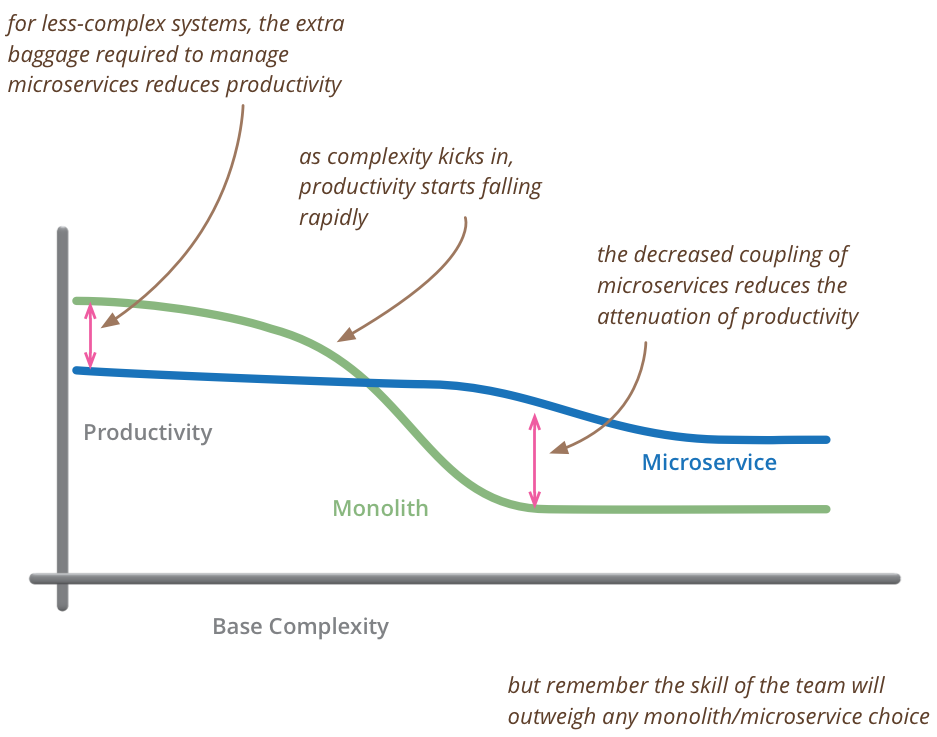
\includegraphics[width=0.7\textwidth]{./images/microservice_architecture/fowler-productivity-complexity.png}
    \caption{Correlation between base complexity and productivity in a microservice architecture compared to a monolithic architecture~\cite{fowlerpremium}}
    \label{fig:fowler_productivity}
\end{figure}

\section{Security Consequences}
The migration to the microservice architecture brings many consequences regarding the security of a deployment.
Especially the network communications among the services introduce a set of vulnerabilities.
Confidentiality, integrity, and availability have to be assured.
The need for authentication mechanisms is a common issue of network security, but the migration from language-level calls to remote calls causes the need for authentication between microservices.
Therefore, the authentication mechanisms discussed in this thesis are a consequence of the microservice architecture and can be neglected with a monolithic architecture.

\chapter{Related Work}
\label{cha:Related_Work}
This chapter summarizes the state-of-the-art concepts for microservice security, public key-based authentication, and the later required technologies.
Service-to-service authentication is only one part of microservice security.
Therefore all related topics, considering microservice security, are discussed.
Furthermore, the concepts of public-key authentication are explained since the authentication mechanisms compared in this thesis are based on public-key cryptography.

\section{Microservice Security}
Siriwardena and Dias~\cite{dias2020microservices} gave an extensive guide of all topics related to microservice security. 
They separated the security of a microservice deployment into edge-level security and service-level security.
Since the microservice architecture splits the backend into multiple minor services, it is insufficient to secure the system only on the edge or service level.
Each part of the system must be appropriately secured regarding confidentiality, authentication, and authorization.

\subsection{Edge-level security}
Edge-level security is defined as the security mechanisms that protect the resources within the deployment from attackers located outside the deployment. 
The API Gateway is responsible for edge security.
It is the only entry point to the microservice deployment.
The API Gateway intercepts all requests targeted for the APIs of the services.
After validating the requests, it dispatches the valid ones to the microservices.
The main tasks of an API Gateway are authentication of the end-user, authorization, and throttling~\cite{dias2020microservices}.
It authenticates the end-user using access tokens, which come from access delegation technologies like OAuth 2.0 or Open ID Connect~\cite{siriwardena2014advanced}.
By outsourcing the end-user authentication to the API Gateway, it has to be performed only once by the API Gateway and not multiple times by each service~\cite{dias2020microservices}.
The API Gateway can perform authorization for all microservices. 
In most cases authorization is performed the edge-level and the service-level. 
The API Gateway performs only coarse authorization assertions, to prevent having a single-point-of-decision~\cite{barabanov2020authentication}.

\subsection{Service-level security}
Service-level security is defined as the security mechanisms that protect the communication among the microservices.
According to Barabanov and Makrushin~\cite{barabanov2020authentication} service-level security can be decomposed into the sub-functions service-level authentication, service-level authorization, and external identity propagation.
Service-level security can either be implemented by the microservices themselves or a service-mesh.
A service mesh can be seen as a dedicated infrastructure layer, which manages the service-to-service communication of containerized services.
In a typical microservice deployment with a service mesh, each microservice has its service proxy, which works transparently~\cite{dias2020microservices}.
The service mesh takes care of service discovery, routing, load balancing, traffic configuration, authentication, authorization, and monitoring~\cite{chandramouli2019microservices}.
Therefore the services can focus on exactly the tasks they are intended for and do not have to care about security-related tasks~\cite{dias2020microservices}.

\subsubsection{Service-to-service-authentication} 
\label{sec:service-to-service-authentication}
Authentication is the process of identifying the communication partner to protect a system from spoofing.
Since the communication among microservices is done using remote calls, their communication has to provide authentication~\cite{dias2020microservices}.
Service-to-service authentication can be implemented in the following ways~\cite{dias2020microservices}:
\begin{itemize}
    \item Trust the Network (TTN)
    \item mutual Transport Layer Security (mTLS)
    \item self signed JSON Web Tokens (JWTs)
\end{itemize}
Trust the Network is a security approach based on the assertion that nobody has access to the components within a network perimeter.
All components rely on network security.
Nevertheless, internal misbehavior can lead to exploits allowing attackers to intrude into the network perimeter and exploit the microservices~\cite{zaheer2019eztrust}. 
Therefore the industry is heading towards zero-trust networks, and the TTN approach is not more used as primary authentication mechanism~\cite{barabanov2020authentication}.

Service-to-service authentication based on mTLS and self-signed JWTs will be discussed in more detail in chapter~\ref{cha:authentication_mechanisms}.

\subsubsection{Service-level authorization} 
\label{sec:service-level-authorization}
Authorization defines the tasks that a principal is allowed to perform on a system.
It requires that the principal is already authenticated because the authorization is performed based on the identity~\cite{siriwardena2014advanced}. 
Service-level authorization gives the microservices more control to enforce access control.
The authorization is usually performed using policy decision point (PDP) models like the centralized PDP model or the embedded PDP model~\cite{dias2020microservices, barabanov2020authentication}.
Proper service-to-service authentication mechanisms are a precondition for service-to-service authorization since the authorization can be bypassed with insufficient authentication~\cite{siriwardena2014advanced}.

\subsubsection{External entity identity propagation} 
\label{sec:external-entity-identity-propagation}
In order to perform the authorization correctly, the services have to know the context of the caller.
The most popular technic for identity propagation is extracting the user's context within JSON Web Tokens.
The tokens are passed between the microservices and the API Gateway.
The propagated identity of the user can be extracted from the token, and the token's signature must be checked.
The microservices can perform authorization based on the identity of the client~\cite{barabanov2020authentication, dias2020microservices}.
The chosen authentication mechanism has an impact on identity propagation. This will be discussed in more detail in chapter~\ref{cha:authentication_mechanisms}.

\section{Public key-Based Authentication}
Authentication can be achieved in multiple ways 
Two common approaches are symmetric cryptography and public-key cryptography.
Both authentication mechanisms discussed in chapter~\ref{cha:authentication_mechanisms} are based on public-key cryptography.
Public key cryptography provides higher security than symmetric cryptography.
Therefore it is the preferred method to implement authentication mechanisms, although it requires higher computation and communication costs than symmetric cryptography~\cite{pubkeycrypto}.

\subsection{Public key cryptography}
Public key cryptography is also called asymmetric cryptography because the main idea is that different keys are used for encryption and decryption~\cite{anderson2020security}.
Each participant is required to own at least one key pair.
A key pair consists of a public key available to everyone and a private key that is only known by the owner of the key pair.
Encrypting a message with the public key allows many people to encrypt messages so that only the person who owns the private key can read them.
Furthermore, it allows one person to encrypt messages in a way that many people can read by encrypting the message with the private key~\cite{henriques2017using}.
This is also known under the term digital signature. 
Digital signatures can be used to provide authentication and integrity for messages~\cite{anderson2020security}.

The commonly used algorithm for digital signatures is RSA.
RSA is based on factoring, its encryption key consists of the modulus $N$, which is hard to factor.
The modulus $N$ is calculated by multiplying the large prime number $p$ and $q$ with each other.
Additionally the encryption key has a public factor $e$ that has no common factors with either $p-1$ or $q-1$.
The private key consists of the factors $p$ and $q$, which have to be kept secret~\cite{anderson2020security}.
The person that knows the private key can encrypt a message using the following formula, where $M$ is the message, and $C$ is the encrypted message~\cite{anderson2020security}:
\begin{displaymath}
	C = M^e (mod N)
\end{displaymath}
An encrypted message can be decryped using the following formular:
\begin{displaymath}
	M = \sqrt[e]{C (mod N)}
\end{displaymath}
Only the owner of the private key can simply calculate the message from the cipher, using the Fermat's little theorem\footnote{See~\cite{fermatlittle} for further information}.

The problem with asymmetric cryptography is that the encryption and decryption times are worse than symmetric cryptography.
The restriction to use only asymmetric cryptography could decrease the system's performance.
Therefore it is common sense to use hybrid systems as done in TLS.
In TLS, public-key cryptography is used for authentication and key exchange, but symmetric cryptography is used to provide confidentiality for the communication~\cite{henriques2017using}.
Henriques~\cite{henriques2017using} showed that the performance of the system can be improved using a hybrid approach.

\subsection{Public Key Infrastructure} \label{sec:pki}
Public key cryptography assumes that the receiver of a message already knows and trusts the sender's public key.
Public Key Infrastructures (PKI) are used to achieve this assertion.
They are responsible for providing a possibility to retrieve the public key of a participant in a trusted way.
This is done using Certificate Authorities (CA) and certificates.
CAs sign certificates, and each communication partner who trusts the CA trusts the certificates signed by it.
For this purpose, usually, X.509 certificates are used~\cite{anderson2020security}.

A PKI can either be an open PKI (global) or a closed PKI (self-hosted).
Closed PKIs have a specific bounded context~\cite{hlavaty2003risk}.
A common use case for closed PKIs is microservice deployments because they are usually company intern and have a specific bounded context~\cite{dias2020microservices}.
The project, which is reviewed in chapter~\ref{cha:project_structure} makes use of a closed PKI created with OpenSSH.
Closed PKIs are a popular option because they allow risk management and provide secrecy of its code.
Open PKIs can be inspected by the public, and based on the inspection, it is determined whether the PKI is trusted or not.
Certificates are retrieved by making partnerships with CAs.
The main advantage is that no proprietary software is needed since the PKIs are managed by the PKI vendors~\cite{hlavaty2003risk}.

\subsection{Key Management} \label{sec:key_management}
Key management is a requirement for public key based authentication. 
It results in being the most challenging part for the later discussed mechanisms.
When the key management is very weak, it will have consequences for all parts of the system.
Especially service-to-service authentication is affected by the quality of the key management.
The authentication mechanism can not stay secure when the keys of the participants are compromised~\cite{dias2020microservices, fumy1993principles}.
According to Fumy et al. ~\cite{fumy1993principles}, a key management service has to implement the following tasks:
\begin{description}
	\item[Entity Registration:] The service must provide a procedure to create a link between an authenticated identity and its keys.
	\item[Key Generation:] The service must provide a procedure to create key pairs with good cryptographic quality.
	\item[Certification:] The service must provide a procedure for issuing certificates. Certification is often a part of key distribution.
	\item[Authentication/Verification:] The service must provide a procedure to guarantee entity authentication, message content authentication, and message origin authentication.
	\item[Key Distribution:] The service must provide a procedure to supply keys for parties legitimately asking for them.
\end{description}

Dias and Siriwardena~\cite{dias2020microservices} furthermore give insights into the key provisioning (distribution) process of Netflix.
Netflix uses its own broker called Lemur for the key provisioning.
It is performed in the following steps, which are visualized in figure~\ref{fig:key_provisioning_netflix}:
\begin{enumerate}
    \item During the continuous delivery process, each microservice gets a set of credentials that are good enough to access the Lemur APIs.
		This is done using a Netflix internal tool called Metatron.
		Metatron credentials are long-lived credentials. 
		They can be used for a longer timer period and the following steps can be repeated multiple times.
    \item The microservice talks to the Lemur API to obtain a signed certificate for its credentials.
		This can happen either during the startup process of the microservice or when the microservice is rotating its keys.
    \item Lemur creates a certificate signing request (CSR) addressed to the CA.
    \item The certificate is signed using the CA.
		Lemur is not a CA, but it knows how to integrate with a CA to generate signed certificates.
    \item Lemur returns the signed certificate to the microservice, who can then use it to authenticate itself to other services.
\end{enumerate}
Therefore the developers do not have to worry about creating and signing certificates.
Instead, they have to implement the communication with the Lemur API.


\begin{figure}
	\centering
	\begin{sequencediagram}
		\newthread{A}{:Microservice}{}
		\newinst[2]{B}{:Metatron}{}
		\newinst[2]{C}{:Lemur}{}
		\newinst[2]{D}{:CA}{}

		\begin{call}{A}{obtain credentials}{B}{credentials}
		\end{call}
		\begin{call}{A}{obtain certificate}{C}{signed certificate}
			\begin{call}{C}{CSR}{D}{signed certificate}
			\end{call}
		\end{call}
	\end{sequencediagram}
	\caption{Key provisioning of netflix using Lemur and Metatron~\cite{dias2020microservices}}
	\label{fig:key_provisioning_netflix}
\end{figure}

%\begin{figure}
%	\centering
%	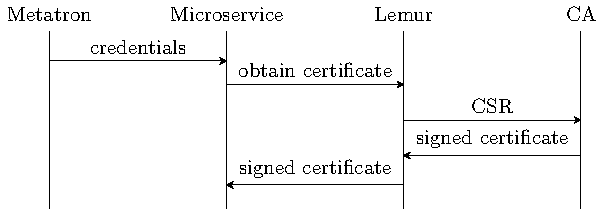
\includegraphics{images/related-work/netflix-provisioning.pdf}
%	\caption{Key provisioning of netflix using Lemur and Metatron~\cite{dias2020microservices}}
%	\label{fig:key_provisioning_netflix}
%\end{figure}

\section{Technologies}
\subsection{X509.Certificate}
X.509 certifcates bind the subject of a certificate to a public key.
They are used to assure the user of a certificate that the certificate's subject owns the corresponding private key.
The most significant advantage of certificates is that they can be exchanged using untrusted communication channels because the signature is not valid anymore when the content of a certificate is changed.
Therefore manipulations can be detected, and manipulated certificates can be declined~\cite{x509rfc}.

When a client wants to consume a service hosted on a server, it has to obtain the server's certificate.
If the client does not know the public key of the CA who signed the server's certificate, he has to obtain it.
Obtaining the public key often results in chains because the client may have to work his way up until he reaches a CA he trusts.
Such chains are also called certification paths~\cite{x509rfc}.

Depending on the version, a certificate can include more or less information.
The information is always stored inside the tbsCertificate, signatureAlgorithm, and signatureValue fields and can be expanded using extensions.
\begin{description}
	\item[TBSCertificate:] contains the data of the certificate, including the subject of the certificate, the issuer of the certificate, the public key of the subject, the validity period, and additional information~\cite{x509rfc}.
	\item[signatureAlogrithm:] stores the information, which cryptographic algorithm was used to sign the certificate.
		Algorithms are declared by their identifier, the "OBJECT IDENTIFIER".
		The most commonly used algorithms are the RSA algorithm and the Digital Signature Algorithm (DSA)~\cite{x509rfc}.
	\item[signatureValue:] contains the value of the digital signature.
		It is obtained by signing the content of the tbsCertificate, using the algorithm specified in the signatureAlgorithm field.
		The signature is used to verify the validity of the information embedded in the tbsCertificate field~\cite{x509rfc}.
\end{description}

\subsubsection{Certificate Revocation}
Certificate revocation is a considerable problem with certificates.
A certificate can be revocated for the following reasons: 
\begin{itemize}
    \item The Private key of the CA is compromised
    \item The Private key of the microservice is compromised
    \item The holder of the certificate is no longer the identity who requested the certificate 
    \item The CA finds out that the parameters provided in the CSR are invalid
\end{itemize}
The hardest part about the certificate revocation is informing all participants about the revocation of a certificate.
This is done using certificate revocation lists (CRL) or other revocation mechanisms.
The big downside of CRLS is that the CA has to store a list of certificates, which are revocated.
The clients have to retrieve this list whenever they establish a connection to a server, which causes high latencies.
The latencies can be reduced by caching.
Otherwise, caching also reduces the security because a certificate can be revocated during the lifetime of the cache.
Especially a case in which the CA does not respond to the CRL query is tough to handle.
Therefore certificate revocation is a significant downside of public-key-based authentication, even if the Online Certificate Status Protocol (OSCP) tries to remedy the situation\cite{dias2020microservices}.


\subsection{JSON Web Token}
A JSON Web Token (JWT) is a container that can carry authentication and authorization assertions and further information in a cryptographically safe manner.
An authentication assertion can be anything that authenticates the user.
Usually, usernames or e-mail addresses are used to identify a user uniquely.
An authorization assertion can be any information about the access permissions of a user.
For example, a JWT can include the information, whether the user is an admin or an unprivileged user~\cite{dias2020microservices}. 

\subsubsection{Structure}
A JWT is decomposed into the header, the payload, and the signature.
The three parts are concatenated and separated by a dot~\cite{jwtdocauth0}.
%A valid JWT could look like the JWT shown in figure~\ref{fig:myjwt}.
%\begin{figure}
%    \textcolor{red}{Header}.
%	\textcolor{blue}{Payload}.
%	\textcolor{darkgreen}{Signature} \\ \\
%    \textcolor{red}{eyJhbGciOiJIUzI1NiIsInR5cCI6IkpXVCJ9}.
%	\textcolor{blue}{eyJzdWIiOiIxMjM0NTY3ODkiLCJpYXQi\\OjE1MTYyMzkwMjIsInVzZXJuYW1lIjoiYmVuamFtaW4uZWxsbWVyIiwiZW1haWw\\iOiJiZW5qYW1pbi5lbGxtZXJAeWFob28uY29tIiwiYWRtaW4iOmZhbHNlfQ}.
%	\textcolor{darkgreen}{0ksqN7\\1oloNvq3IrY7w72uoTgPz9Gpn08p-KSbFulY0}
%    \caption{Sample JSON Web Token}
%    \label{fig:myjwt}
%\end{figure}

The \textbf{header} contains metadata related to the JWT, which is usually the type of the token and the signature algorithm.
The specification defines that only HS256\footnote{HMAC SHA-256} and none algorithm must be implemented by conforming JWT implementation.
It is recommended to additionally implement the algorithms RS256 and ES256\footnote{Elliptic Curve Digital Signature Algorithm (ECDSA) with 256-bit key}~\cite{jwtdocauth0, jwtrfc}.
The base64 encoded header is the first part of the JWT.

The \textbf{payload} is a set of registered and custom claims.
A claim is a piece of information about an entity.
The JWT specification defines registered claims, which are not mandatory for all cases but should provide a good starting point for a set of valuable claims to ensure interoperability.
The software architects can define custom claims on their own, depending on their needs.
The custom claims registered in the IANA registry are called public claims, and those not registered in the IANA registry are called private claims~\cite{jwtdocauth0, jwtrfc}.
The base64 encoded payload is the second part of the JWT.

The chosen signature algorithm signs the base64 encoded header, the base64 encoded payload, and a secret (only with symmetric encryption like HMAC).
The \textbf{signature} provides integrity for the message, and if it was signed with a private key, it additionally provides authentication~\cite{jwtdocauth0}.
The base64 encoded signature is the third part of the JWT.

\subsection{Transport Layer Security}
The Transport Layer Security (TLS) Protocol provides authentication, integrity, and confidentiality for the communication between two parties.
It consists of two layers, the handshake protocol and the record protocol~\cite{turnertls}.

\subsubsection{Handshake Protocol}
The handshake protocol is responsible for negotiating a cipher suite and for providing authentication using X.509 certificates.
The cipher suite declares the key exchange algorithm, the signature algorithm, the symmetric encryption algorithm, including the mode of the encryption algorithm and the hashing algorithm~\cite{turnertls, kurbatov2021design}.
The handshake varies on the key exchange method, but it can be separated into the following steps~\cite{krawczyk2013security}:
\begin{enumerate}
    \item The server and the client exchange Hello messages.
    \item The server sends its certificate to the client.
    \item The client sends a pre-master secret to the server.
    \item The client and the server finish the handshake, using the independently computed master secret.
\end{enumerate}

\subsubsection{Record Protocol}
The record protocol provides a secure channel for the secure communication of two parties.
This is done by using the algorithms declared in the cipher suite.
Confidentiality is assured, using symmetric encryption, and Message Authentication Codes (MAC) provide integrity~\cite{kurbatov2021design, krawczyk2013security}.

\subsubsection{mTLS} \label{sec:mtls}
TLS itself is also called one-way TLS because it helps the client to identify the server, but not the server to identify the client.
Therefore mTLS was introduced to provide authentication in both directions.
The client and the server must own a private/public key pair, so it is more suited for the communication between two systems and not between users and servers~\cite{dias2020microservices}. 
The authentication of the client is performed during the handshake.
When mTLS is used, the client has presents his certificate to the server, before transferring the pre-master secret.

\section{Conclusion}
This chapter described the fundamentals to understand the details and differences between the later described authentication mechanisms.
Furthermore, it was described why service-to-service authentication is needed and what additional mechanisms have to be implemented to secure a microservice deployment.

It is essential to understand that the whole system is compromised when one security mechanism does not work correctly.
For example, the authorization can be affected when the authentication is neglected.
Each service and each layer of the deployment has to be appropriately secured.
The problem with the microservice architecture is that one compromised service can be used to compromise other services.
Therefore, choosing the correct security mechanisms and understanding how they work is crucial. 

%Additionally, the possibility of outsourcing the authentication to a service mesh was discussed.
%The authentication mechanisms stay the same regardless of whether they are performed bythe services themselves or using the service mesh pattern.
%For the simplicity, it is assumed that the authentication mechanisms are performed by the services themselves in the following chapters.

%\chapter{Technologies}
This chapter describes the technologies and tools, which are necessary for the implementation of the later discussed authentication mechanisms.

\section{X509.Certificate}
X.509 certificates assure the users of a public key that the associated person or system owns the private key by binding public keys to subjects.
Certificate authorities sign certificates and each communication partner who trusts the CA trusts the certificates signed by it.
The most significant advantage of certificates is that they can be exchanged using untrusted communication channels because the signatures are not valid anymore when the contents of a certificate are changed.
Therefore manipulations can be detected, and manipulated certificates can be declined~\cite{x509rfc}.

\subsection{Trust Path}
When the client of a service wants to consume a service, which is hosted on a server, it has to obtain the server's certificate.
If the client does not know the public key of the CA who signed the server's certificate, he has to obtain it.
Obtaining the public key often results in chains because the client may have to work his way up until he reaches a CA he trusts.
Such chains are also called certification paths.
The way in which the clients can retrieve the CA certificates can be configured by the CA.

\subsection{Fields}
Depending on the version, a certificate can include more or less information.
The information is always stored inside the tbsCertificate, signatureAlgorithm, and signatureValue fields and can be expanded using extensions.

\subsubsection{TbsCertificate}
The TBSCertificate contains the data of the certificate, including the following information:
\begin{itemize}
    \item Subject of the certificate
    \item Issuer of the certificate
    \item public key of the subject
    \item Validity period
    \item Additional information
\end{itemize}

\subsubsection{SignatureAlgorithm}
The signatureAlogrithm field stores the information, which cryptographic algorithm was used to sign the certificate.
Algorithms are declared by their identifier, the "OBJECT IDENTIFIER".
The most commonly used algorithms are the RSA\footnote{Rivest Shamir Adleman} algorithm and the Digital Signature Algorithm (DSA)~\cite{x509rfc}.

\subsubsection{SignatureValue}
The signatureValue field contains the value of the digital signature.
It is obtained by signing the content of the tbsCertificate, using the algorithm specified in the signatureAlgorithm field.
The signature is used to verify the validity of the information embedded in the tbsCertificate field.

\section{JSON Web Token}
A JSON Web Token (JWT) is a container, which can carry authentication and authorization assertions and further information in a cryptographically safe manner.
An authentication assertion can be anything, which authenticates the user.
Usually, usernames or e-mail addresses are used to identify a user uniquely.
An authorization assertion can be any information about the access permissions of a user.
For example, a JWT can include the information, whether the user is an admin or an unprivileged user~\cite{dias2020microservices}. 

\subsection{Structure}
A JWT is decomposed into the header, the payload, and the signature.
The three parts are concatenated and separated by a dot~\cite{jwtdocauth0}.
A valid JWT could look like the JWT shown in figure~\ref{fig:myjwt}.
\begin{figure}[H]
    \textcolor{red}{Header}.
	\textcolor{blue}{Payload}.
	\textcolor{darkgreen}{Signature} \\ \\
    \textcolor{red}{eyJhbGciOiJIUzI1NiIsInR5cCI6IkpXVCJ9}.
	\textcolor{blue}{eyJzdWIiOiIxMjM0NTY3ODkiLCJpYXQi\\OjE1MTYyMzkwMjIsInVzZXJuYW1lIjoiYmVuamFtaW4uZWxsbWVyIiwiZW1haWw\\iOiJiZW5qYW1pbi5lbGxtZXJAeWFob28uY29tIiwiYWRtaW4iOmZhbHNlfQ}.
	\textcolor{darkgreen}{0ksqN71\\oloNvq3IrY7w72uoTgPz9Gpn08p-KSbFulY0}
    \caption{Sample JSON Web Token}
    \label{fig:myjwt}
\end{figure}

\subsubsection{Header}
The header contains the metadata related to the JWT, which is usually the type of the token and the signature algorithm.
The specification defines that only HS256\footnote{HMAC SHA-256} and none algorithm must be implemented  by conforming JWT implementation.
It is recommended to additionally implement the algorithms RS256 and ES256\footnote{Elliptic Curve Digital Signature Algorithm (ECDSA) with 256-bit key}~\cite{jwtdocauth0, jwtrfc}.
The base64 encoded header is the first part of the JWT.

\subsubsection{Payload} 
The payload is a set of registered and custom claims.
A claim is a piece of information about an entity.
The JWT specification defines registered claims, which are not mandatory for all cases but should provide a good starting point for a set of useful claims to ensure interoperability.
Custom claims can be defined by the software architects, on their own, depending on their needs.
The custom claims registered in the IANA registry are called public claims, and those not registered in the IANA registry are called private claims~\cite{jwtdocauth0, jwtrfc}.
The base64 encoded payload is the second part of the JWT.

\subsubsection{Signature}
The chosen signature algorithm signs the base64 encoded header, the base64 encoded payload, and a secret.
The signature provides integrity for the message, and if it was signed with a private key, it provides authentication~\cite{jwtdocauth0}.
The base64 encoded signature is the third part of the JWT.

\section{Transport Layer Security}
The Transport Layer Security (TLS) Protocol provides authentication, integrity, and confidentiality for the communication between two parties.
It consists of two layers, the handshake protocol, and the record protocol~\cite{turnertls}.

\subsection{mTLS} \label{sec:mtls}
TLS itself is also called one-way TLS because it helps the client to identify the server, but not the server to identify the client.
Therefore mutual TLS (mTLS) was introduced to provide authentication in both directions.
The client and the server must own a private/public key pair, so it is more suited for the communication between two systems and not between users and servers~\cite{dias2020microservices}. 

\subsection{Handshake Protocol}
The handshake protocol is responsible for negotiating a cipher suite and for the authentication using X.509 certificates.
The cipher suite declares the key exchange algorithm, the signature algorithm, the symmetric encryption algorithm, including the mode of the encryption algorithm and the hashing algorithm~\cite{turnertls, kurbatov2021design}.
The handshake varies on the key exchange method, but it can be separated into the following steps~\cite{krawczyk2013security}:
\begin{enumerate}
    \item The server and the client exchange Hello messages
    \item The server sends its certificate to the client
    \item The client sends a pre-master secret to the server and if mTLS is used, the client sends his certificate to the server
    \item The client and the server finish the handshake, using the independently computed master secret
\end{enumerate}
The steps of the handshake will be explained in more detail in chapter~\ref{sec:tlshandshake_details}.

\subsection{Record Protocol}
The record protocol provides a secure channel for the communication between the parties.
This is done by using the algorithms declared in the cipher suite.
Confidentiality is assured, using symmetric encryption, and integrity is provided by Message Authentication Codes (MAC)~\cite{kurbatov2021design, krawczyk2013security}.

%\section{OpenSSL}
%OpenSSL is an open-source library that provides implementations of the state-of-the-art cryptographic algorithms, including the TLS protocols.
%It is fully cross-platform and can either be used within programs or by its CLI.
%It is crucial to use libraries like OpenSSL for cryptographic operations because most developers are not fully aware of all dangers, resulting in vulnerabilities caused by faulty implementations~\cite{viega2002network}.
%OpenSSL will be used to create and sign keys and certificates in chapter~\ref{cha:Implementation}.

%\subsection{OpenSSL file formats}
%Files with the following extensions are created and used in chapter~\ref{cha:Implementation}.
%The file extensions are not exclusive to the OpenSSL library, and these are only the extensions that are later used.
%There are many more available extensions, which are not discussed in this thesis~\cite{opensslextensions, viega2002network}:
%\begin{description}
%    \item[pem:] A Privacy Enhanced Mail file is a base64 encoded text file, which can be used as a container for a private key, or one to many certificates.
%    \item[crt:] A pem file containing certificates can use the crt extension instead of the pem extension.
%    \item[key:] A pem file containing a private key can use the key extension instead of the pem extension.
%    \item[csr:] A csr file contains a certificate signing request intended to be signed by a certificate authority.
%    \item[pfx:] A pfx file is a container that can include certificates and a private key together in a binary file.
%\end{description}

\chapter{Authentication Mechanisms}
\label{cha:authentication_mechanisms}
This chapter explains the concepts and details of the two compared authentication mechanisms.
Only the mTLS approach and the authentication using self-signed JWTs approach are discussed in this chapter, since the Trust the Network (TTN) approach is deprecated and should not be used anymore.

\begin{figure}
	\centering
	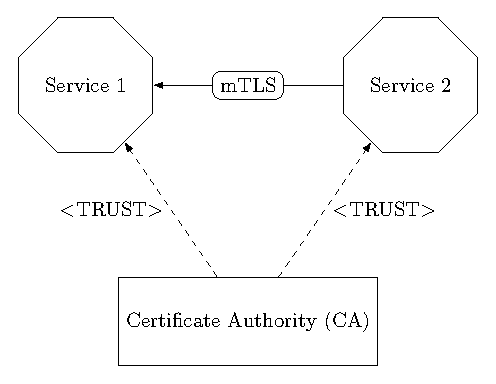
\includegraphics{images/authentication-mechanisms/TikZ_mTLS_base_structure.pdf}
	\caption{Setup using mTLS for the service-to-service authentication~\cite{dias2020microservices}}
	\label{fig:auth_mechanisms_mtls}
\end{figure}

\section{Authentication based on mTLS}
Mutual TLS is the most popular option for the service-to-service authentication of microservice deployments~\cite{dias2020microservices}.
Securing the communication with TLS already provides integrity, confidentiality and furthermore authenticates the server to the client.
Since basic TLS does not provide authentication from the client to the server, it is not sufficient for the service-to-service security.
Therefore mutual TLS is used, which provides an efficient and straightforward approach to authenticate the client to the server.

The authentication using mTLS requires a PKI, same as the authentication using basic TLS.
It is possible to use the already existing PKI of the internet, but this would make the key management much harder and would not bring any advantages.
% TODO: Insert Reference to self hosted PKI
Therefore it is good practise to use a self-hosted PKI to have a root of trust within the network~\cite{dias2020microservices}.
The setup of a microservice deployment using mTLS is shown in figure~\ref{fig:auth_mechanisms_mtls}.

When mTLS is used, both the server and the client must provide a valid certificate to create a communication channel.
The issuer of the presented certificates must be trusted by all communicating parties~\cite{dias2020microservices}.
If one communication partner does not have a valid certificate, the communication is neglected.
Therefore each service needs his own private key, and the corresponding public key.
Additionally a signed certificate, which binds the public key to the subject of the certificate, is needed.
The certificates of the communication partners are exchanged during the TLS handshake.

This mechanism can also be used to authenticate the end users of an application.
For this context the term Client Certificate Authentication (CCA) is used.
The service-to-service authentication using mTLS is a implementation of CCA, but in this approach the client is not the end user, instead it is another service.

\subsection{Handshake}
\label{sec:tlshandshake_details}
The handshake is used to exchange the certificates of the participants and setup the connection.
The steps of the handshake differ between the used algorithms and versions of the TLS protocol.
The following sequence and figure~\ref{fig:tlshandshake} should give an overview about the steps of the TLS handshake using mutual TLS~\cite{parsovs2013practical}:
\begin{enumerate}
	\item The client initializes the connection by sending a \textbf{ClientHello} message to the server.
		The \textbf{ClientHello} message includes a list of supported cipher suits, and the randomness, which is a combination of random bytes and the current date~\cite{mediumtls}.
	\item The sever responds with a \textbf{ServerHello}, in which he chooses one cipher suite of the \textbf{ClientHello} message.
		Furthermore the \textbf{ServerHello} contains the servers randomness.
	\item The server sends the \textbf{Certificate} messages, containing one or more certificates, which can be used to build the certificate chain.
		The client validates the sent certificates with his own trusted store.
		If the trusts the sent certificate chain, the server is successfully authenticated.
	\item The server sends the \textbf{CertificateRequest} message, in which the trusted CAs of the server are listed.
		The client can use this list to choose the correct certificate he has to present.
	\item The server sends the \textbf{ServerHelloDone} message.
	\item The client responds with his \textbf{Certificate} message, which is similiar to the servers \textbf{Certificate} message, but contains the client's certificate chain.
	\item The client then generates a random value the pre-master secret.
		The pre-master secret is used to derive symmetric keys for the cryptographic operations defined in the cipher suite.
		Then the pre-master secret is encrypted, using the public key of the server.
		Therefore, only the owner of the corresponding private key, which is the server can decrypt this message.
		In the end the encrypted pre-master secret is transferred to the server within the \textbf{ClientKeyExchange} message.
	\item The client has to proove that he owns the corresponding private key of the certificate he sent.
		Therefore he has to encrypt the hash of all previous messages with his private key.
		This encrypted hash is then sent to the server within the \textbf{CertificateVerify} message.
		The sever can decrypt the hash with the public key of the certificate and can calculate the hash on his own to check whether the decrypted hash is correct or not.
	\item The client sends a \textbf{ChangeCipherSpec} message, to signal the server, that all following messages will be protected with the protection mechanisms defined in the cipher suite.
	\item The last message of the handshake is the \textbf{Finished} message, which is an encrypted hash of all previous messages.
	\item Same as step 9, but from the server.
	\item Same as step 10, but from the server.
\end{enumerate}
After the handshake both participants know the secret, which can be used to encrypt and decrypt messages.
The handshake would have almost the same steps when mTLS is not used.
Only the \textbf{CertificateRequest} message of the sever and the \textbf{Certificate} message and the \textbf{CertificateVerify} message of the client are unique for mTLS.
One special case of the handshake is, that the client responds to the \textbf{CertificateRequest} with a empty \textbf{Certificate} message.
Depending on the configuration of the server, the connection without a certificates can be allowed or neglected~\cite{parsovs2013practical}.

\begin{figure}
    \centering
	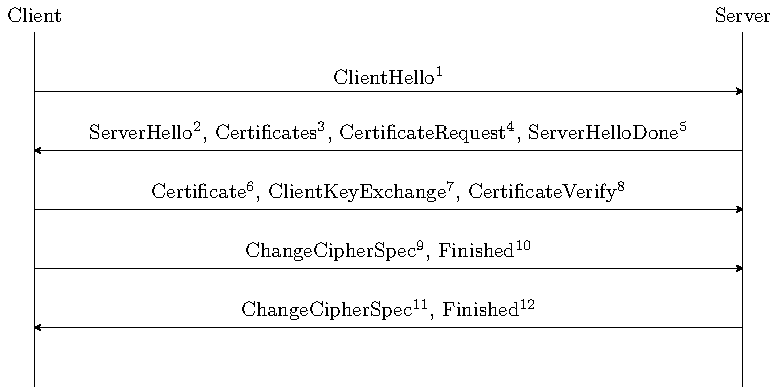
\includegraphics{authentication-mechanisms/TikZ_handshake.pdf}
    \caption{TLS handshake using mTLS~\cite{parsovs2013practical}}
	\label{fig:tlshandshake}
\end{figure}

\subsection{Passing the end user context}
For some functionalities, the identity of the microservice is not relevant, instead the identity of the end user is relevant.
In those cases, the microservices have to pass the end user context, when they consume the logic of other microservices.
The most popular approach for passing the end user context with mTLS are JSON Web Tokens.
This approach can be implemented in multiple ways~\cite{dias2020microservices}.

Genereally, the user obtains a access token from any token service.
This token could be a OAuth2, an OpenID Connect token or any other token.
The user has to send this token with each request.
The token is than validated by a Security Token Service (STS).
If the token is valid, the STS returns a JWT, which can then be used to consume other services.
When one microservice calls another microservice he sends the JWT and if this microservice has to consume another microservice, he also passes the same token to the next microservice~\cite{dias2020microservices}.
The workflow of this approach is shown in figure~\ref{fig:mtls_id_1}
\begin{figure}
    \centering
	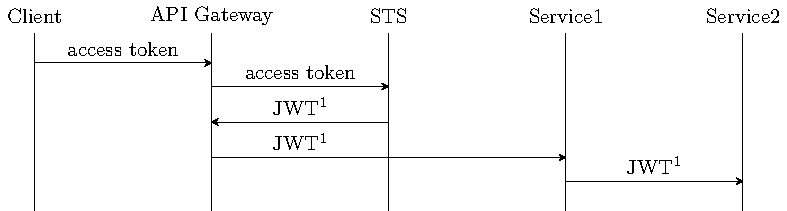
\includegraphics{images/authentication-mechanisms/TikZ_jwt_identity_1.pdf}
    \caption{Use the same JWT for each request~\cite{dias2020microservices}}
	\label{fig:mtls_id_1}
\end{figure}

Another approach is, that the STS is used to generate a new token for each request like it is shown in figure~\ref{fig:mtls_id_2}.
When the STS generates a new token for each request, he has full knowledge about all performed requests.
Therefore the STS could implement further authorization logic.
But the frequent calls could result in a enourmous workload for the STS and could decrease the performance of the system.

\begin{figure}[H]
	\centering
	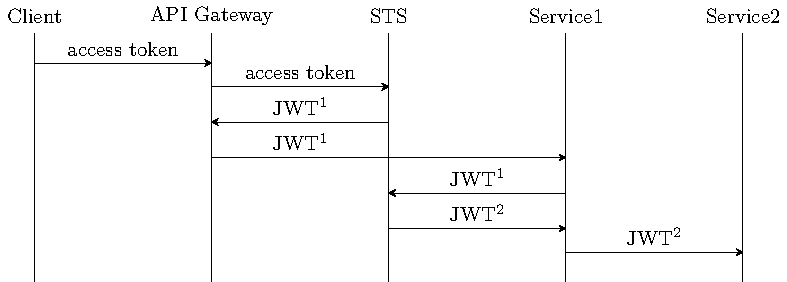
\includegraphics{images/authentication-mechanisms/TikZ_jwt_identity_2.pdf}
	\caption{Generate new JWT for each request~\cite{dias2020microservices}}
	\label{fig:mtls_id_2}
\end{figure}

Both approaches result in some overhead, especially the second approach.
Additionally, when the microservices are located in different trust domains, those approaches can get very complicated, since a microservice only trusts the STS within his trust domain~\cite{dias2020microservices}.
Therefore, mTLS might not be the superior approach for systems, which require the services to know the end user context.

\subsection{Conclusion}
mTLS is a efficient mechanism to implement service to service authentication.
Since the communication between the services is usually done using HTTPS, the services already use TLS.
Therefore the use of mTLS does not cause much configuration overhead and no new technologies are necessary~\cite{dias2020microservices}, unless the services have to share the end user context.

One crucial advantage of the TLS handshake is that the private keys are never exchanged and the session keys are always different, due to the usage of the randomness.
This means even if an intruder is able to get the session key of a communication channel, he is not able to use this key for another session.
Furthermore it is not possible to retrieve any information about the private key of the communication partners with the knowledge of the session key.
This shows how secure mTLS is, even for advanced attacks~\cite{parsovs2013practical}.

From the developer perspective, mTLS does not require to implement much logic.
The service which acts as the server has to be configured to use certificate authentication.
Depending on the used technologies, this is usually done by setting a few configuration parameters in the code, or directly on the webserver.
The service which acts as the client has to be configured to send his certificate during the TLS handshake.
Most HTTP Client libraries support to simply attach the certificate to each HTTP Request.
But the fact that the developers do not have to implement much logic, results in the problem, that they do not have much control about the system.
The developers have to rely on the implementation of the webserver developers.
This means if a webserver has security related bugs, the microservice developers can not solve them on their own.
For example the apache webserver, which is one of the most popular webservers had many issues, in combination with CCA.
Arnis Parsovs~\cite{parsovs2013practical} researched about the problems of the apache webserver and gave an exhensive guide how to circumvent all bugs, when CCA is configured.

% TODO: Referenz auf key management
The biggest challenge of mTLS is the key management, which was described in more detail in chapter.
Key management is responsible for key provisioning, key revocation, key rotation and some more management tasks.
Usually the key management results in requiring a self-hosted PKI for the deployment.
For small applications the key management can be kept very simple.
But as soon as the deployment grows and many services are running at the same time, automation tools are required.
Therefore the management overhead of mTLS is much harder to handle, than the implementation of mTLS itself~\cite{dias2020microservices}.

The previous mentioned challenges and motivation result in the conclusion that mTLS is a very useful and efficient approach, when the developers do not require to fully control each aspect of the authentication.
Especially, when the end user context has to be shared among the services, mTLS might not be the most efficient solution.
Even if mTLS may not be the ultimate tool for all security challenges, in regard with service-to-service authentication, it does its job and it does it well.
This is the reason why mTLS is the most pupular approach for service-to-service authentication.

\section{Authentication based on self signed JWTs}

\chapter{Project Structure}
\label{cha:project_structure}
This chapter shows the structure of an project which implements the previously discussed authentication mechanisms.
This chapter aims to clarify the interactions of the components which are needed to implement the service-to-service security.
The visualizations of this chapter are based on a microservice backend for a flea market app.
The backend is implemented in C\# using the ASP.NET framework.

\section{Components}
The components of the example deployment are shown in figure~\ref{fig:deployment_structure}. 
It consists of the following parts:
\begin{description}
	\item[Android App:] The Android App is the User Interface for the client to access the functionalities of the service.
		The requests sent by the Android App are sent in beyond of the user.
	\item[Firebase Authentication:] The Firebase Authentication service is responsible for validating the access tokens wich are transferred by the users.
	\item[API Gateway:] The API Gateway is the only entry point to the deployment.
		Therefore the API Gateway is the only component which directly communicates to the Android App.
	\item[AdService:] The AdService is one service of the deployment.
		It is responsible to manage all ads offered to the users of the app.
	\item[UserService:] The AdService is the service which is responsible for managing the data of the users.
\end{description}

\begin{figure}
	\centering
	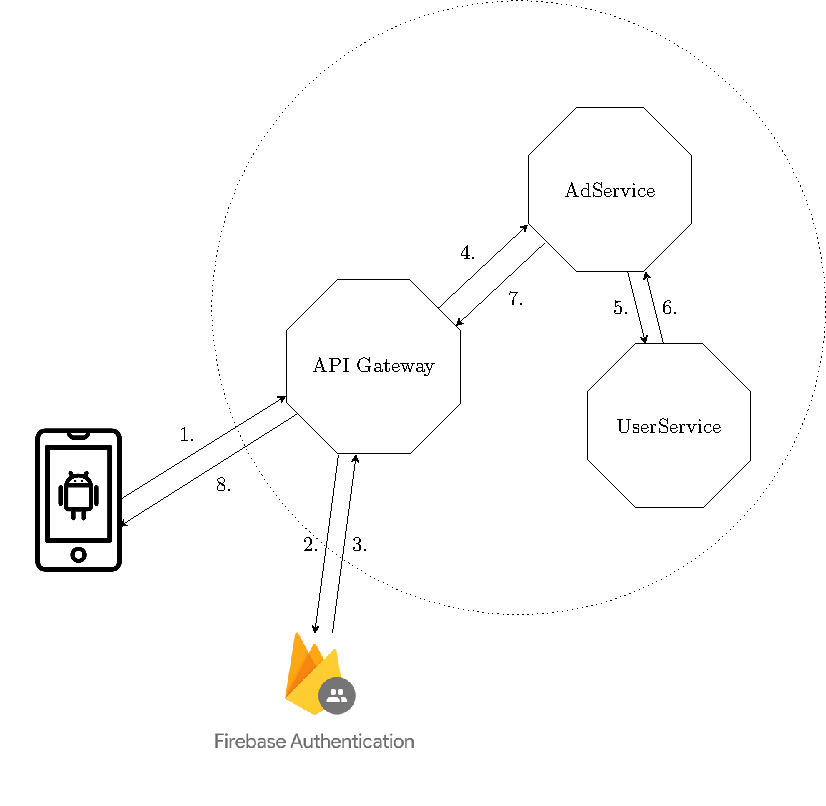
\includegraphics{images/project-structure/TikZ_structure.pdf}
	\caption{Structure of the deployment}
	\label{fig:deployment_structure}
\end{figure}

\section{Workflow using mTLS}

\begin{enumerate}
	\item The client sends an API request to the Microsoft API Gateway using an Android App.
		The client communicates with the API Gateway using HTTPS.
		Therefore the server is authenticated to the client using TLS.
		The client is authenticated to the server by embedding an firebase access token within the Authorization header.
	\item The API Gateway receives the request from the client and has to check the provided access token.
		The token is validated using an token validation service provided by firebase.
		If the token is invalid, the client has to retrieve a new token an start from the beginning.
		When the client provided an valid access token, the request of the client is forwarded to the "AdService".
		The communication between the API Gateway and the "AdService" is secured using mTLS.
		This means both the API Gateway and the AdService have to present a valid certificate signed by a trusted CA.
	\item The request from the client is then processed on the "AdService".
		Since the "AdService" needs information about the users which are the owners of the ads, it needs to communicate with the "UserService".
		The communication between the "UserService" and the "AdService" is also protected using mTLS.
	\item When the "UserService" processed the request from the "AdService", it responds with the expected result.
		The response does not require to present the certificates again, since TCP connection between the "AdService" and the "UserService" is still present.
	\item The "AdService" then processes the response from the "UserService" and sends its request to the API Gateway, again using the opened TCP connection.
	\item The API Gateway forwards the response from the "AdService" to the Android App.
		This connection is still secured using TLS and not mTLS.
		It would be possible to secure the communication between the API Gateway and the client using certificate.
		This mechanism is called Client Certificate Authentication.
	\item The App can now process the response and present the requested information to the user.
\end{enumerate}

\section{Workflow using self signed JWT}

\chapter{Experiment}
\label{cha:experiment}
This chapter discusses an experiment, that measures the performance of the previously described authentication mechanisms.
Even if the performance is not the major decision point to choose the correct authentication mechanism, it is still worth considering it.
Especially, because the migration from a monolithic architecture to the microservice architecture already results in a massive performance decrease of around 79.1\%~\cite{ueda2016workload}.
Therefore the performance is already restricted, and the authentication mechanisms should not produce too much overhead.

\section{Setup}
The setup consists of two components, the service, that responds to requests and the client, which performs requests and measures the taken time.
Both components are located in the same network and run on the same machine.
The service is developed in C\# using ASP.Net Core, same as the services of the flea market app, mentioned in chapter~\ref{cha:project_structure}.
The client is a console application, developed in C\# using .NET.
It is not a microservice, but it acts as a service that is located within the deployment.
In a usual deployment it is not good practice to access the services directly from an external application, bypassing the API Gateway.
Nevertheless, for the purpose of an experiment, this is allowed to make the setup simpler and reduce falsifications by other components. 

%The experiment consists of two test cases.
%In the first test case (case A), the console application fetches random numbers from the service.
%Therefore the service does not have to establish any connection to a database.
% TODO: geht das nicht besser ?
%The absolute duration of this test case will not be very meaningful, because it is very unrealistic, that a service considers another service for a task like creating a random number.
%But the trend of this times gives a good value for the comparison of the authentication mechanisms, since the falsification of other operations like accessing a database is minimized.
%In the second case (case B), the console application fetches all users stored in a database table.
%The difference between the two test cases will show how much time has is accounted to the authentication mechanisms and how much time is accounted to other tasks.

The experiment simulates the situation that a service (the console application) performs 1000 requests to another service.
The connection between the console application and the service has to be established, when the first request is performed.
Therefore the first request will take significantly longer, since the full TCP handshake and TLS handshake have to be performed.
Following requests can reuse the already created connection and do not have to perform the whole initialisation process again.
The tests were performed five times to minimize distortions between the test runs.

This experiment does not aim to give and approximation of the expected request durations with the declared technology stack.
Instead it will compare the trends between the authentication mechanisms.
The exact durations are not relevant, since they are influenced by many factors, like the hardware of the components.

Two different implementations of the approach using self-signed JWTs are compared to the performance using mTLS.
First, an implementation of the self-signed JWT approach, in which a new JWT is created for each request is shown.
The second implementation uses the same JWT for all requests.
This should give an idea how the performance using self-signed JWTs can be improved by efficiently reusing the tokens.
Furthermore the experiment includes the response duration without using any authentication mechanism.
This should show how much time is accounted for the authentication mechanisms and how much time is accounted for other tasks like the transport of the request or the generation of the random number.

To simplify the interpretation of the results, the approaches are identified using the identifiers declared in table~\ref{tab:experiment_case_1}.
%\begin{itemize}
%	\item mTLS $\rightarrow \alpha$
%	\item self-signed JWT $\rightarrow \beta$
%	\item self-signed JWT (reusing token) $\rightarrow \gamma$
%	\item none $\rightarrow \delta$
%\end{itemize}
%\begin{table}[H]
%	\centering
%	\begin{tabular}{c|c}
%		\textbf{Authentication Mechanism} & \textbf{Identifier} \\ \hline
%		mTLS & $\alpha$ \\ \hline
%		self-signed JWT & $\beta$ \\ \hline
%		self-signed JWT (reusing token) & $\gamma$ \\ \hline
%		none & $\delta$ \\
%	\end{tabular}
%	\caption{Identifiers for the compared approaches}
%	\label{tab:identifiers}
%\end{table}

\section{Results}

\begin{table}[H]
	\centering
\begin{tabular}{c|c|cc}
	\multicolumn{1}{l|}{\textbf{Authentication Mechanism}} & \textbf{Identifier} & \multicolumn{2}{c}{\textbf{Average Request Duration}} \\ \hline
	\multicolumn{1}{c|}{} & & \multicolumn{1}{c|}{first connection} & reuse connection \\ \hline
	mTLS & $\alpha$ & \multicolumn{1}{c|}{$228.03$ ms} & $9.87$ ms \\ \hline
	self-signed JWT & $\beta$ & \multicolumn{1}{c|}{$193.52$ ms} & $13.57$ ms \\ \hline
	self-signed JWT (reusing token) & $\gamma$ & \multicolumn{1}{c|}{$184.88$ ms} & $8.10$ ms \\ \hline 
	none & $\delta$ & \multicolumn{1}{c|}{$175.78$ ms} & $1.31$ ms
\end{tabular}
\caption{Average request durations of the authentication mechanisms, when random numbers are fetched}
\label{tab:experiment_case_1}
\end{table}

The results of the experiment are shown in table~\ref{tab:experiment_case_1}.
Furthermore the trend of the average request durations is visualized in figure~\ref{fig:trend}.

According to the experiment results $\delta$ is the most efficient approach, because it does not have to handle any additional authentication mechanism.
The first request takes only 175.78 ms in average and the following requests take only 1.31 ms in average.
Comparing $\delta$ with $\alpha$ shows that $\alpha$ takes in average 8.56 ms longer than $\delta$ resulting in a 750\% increase.
Since the authentication is performed only once per request it is not valid to say that the request duration between $\delta$ and $\alpha$ increases by 750\%.
The percentual value is only such significant because the task of generating a random number is very simple.
Therefore only the time offsets of this comparison are interesting.
They show that $\alpha$ increases the request duration by about 8.56 ms on average compared to $\delta$.
The approaches using self-signed JWTs increase the average request duration by 6.79 ms ($\gamma$) to 12.26 ms ($\beta$) on average compared to $\delta$. 

When service-to-service authentication is provided, the lowest duration to establish the first connection is achieved using $\gamma$.
This is reasonable, since $\alpha$ has to perform the extended TLS handshake to transfer the certificate and proove that it owns the corresponding private key.
When self signed-JWTs are used, the services have to proove that they own the private key of the transferred certificate by signing the JWTs.
Therefore the extended handshake is not necessary, for the approaches $\beta$ and $\gamma$.
The results show that $\alpha$ takes about 52.52 ms longer in average than $\gamma$ for establishing the first connection with a service.
$\gamma$ has a minimal advantage of 8.64 ms in average for establishing the first connection compared to $\beta$, because it does not have to create a JWT.

% fake news
%When service-to-service authentication is provided, the lowest duration for the first connection is achieved using mTLS. 
%This is reasonable, since the authentication using self-signed JWTs exchanges the certificate of the client in the first request using the extended TLS handshake same as mTLS.
%Therefore in all three cases the extended TLS handshake has to be performed but the JWT approaches have to attach the JWT additionally.
%The approach that reuses a previously created JWT needs about 10 ms less than the approach in which an new JWT has to be created.
%The first connection using an already created JWT takes still around 16 ms more than the first connection using mTLS.
%This time overhead is caused by the logic that checks the certificate and stores it into the truststore and then checks the validity of the JWT.

Considering the requests after the connection was established, $\gamma$ is the most efficient approach except $\delta$, which does not provide authentication.
Each request takes about 8.10 ms in average which is about 1.23 ms less than using $\alpha$ and 5.47 ms less than $\beta$.
Nevertheless in a more realistic example it is not possbile to reuse the same token for each request.
Therefore using self-signed JWTs would result in a request duration between $\beta$ and $\gamma$ which is around the request duration of $\alpha$.

\begin{figure}
	\centering
	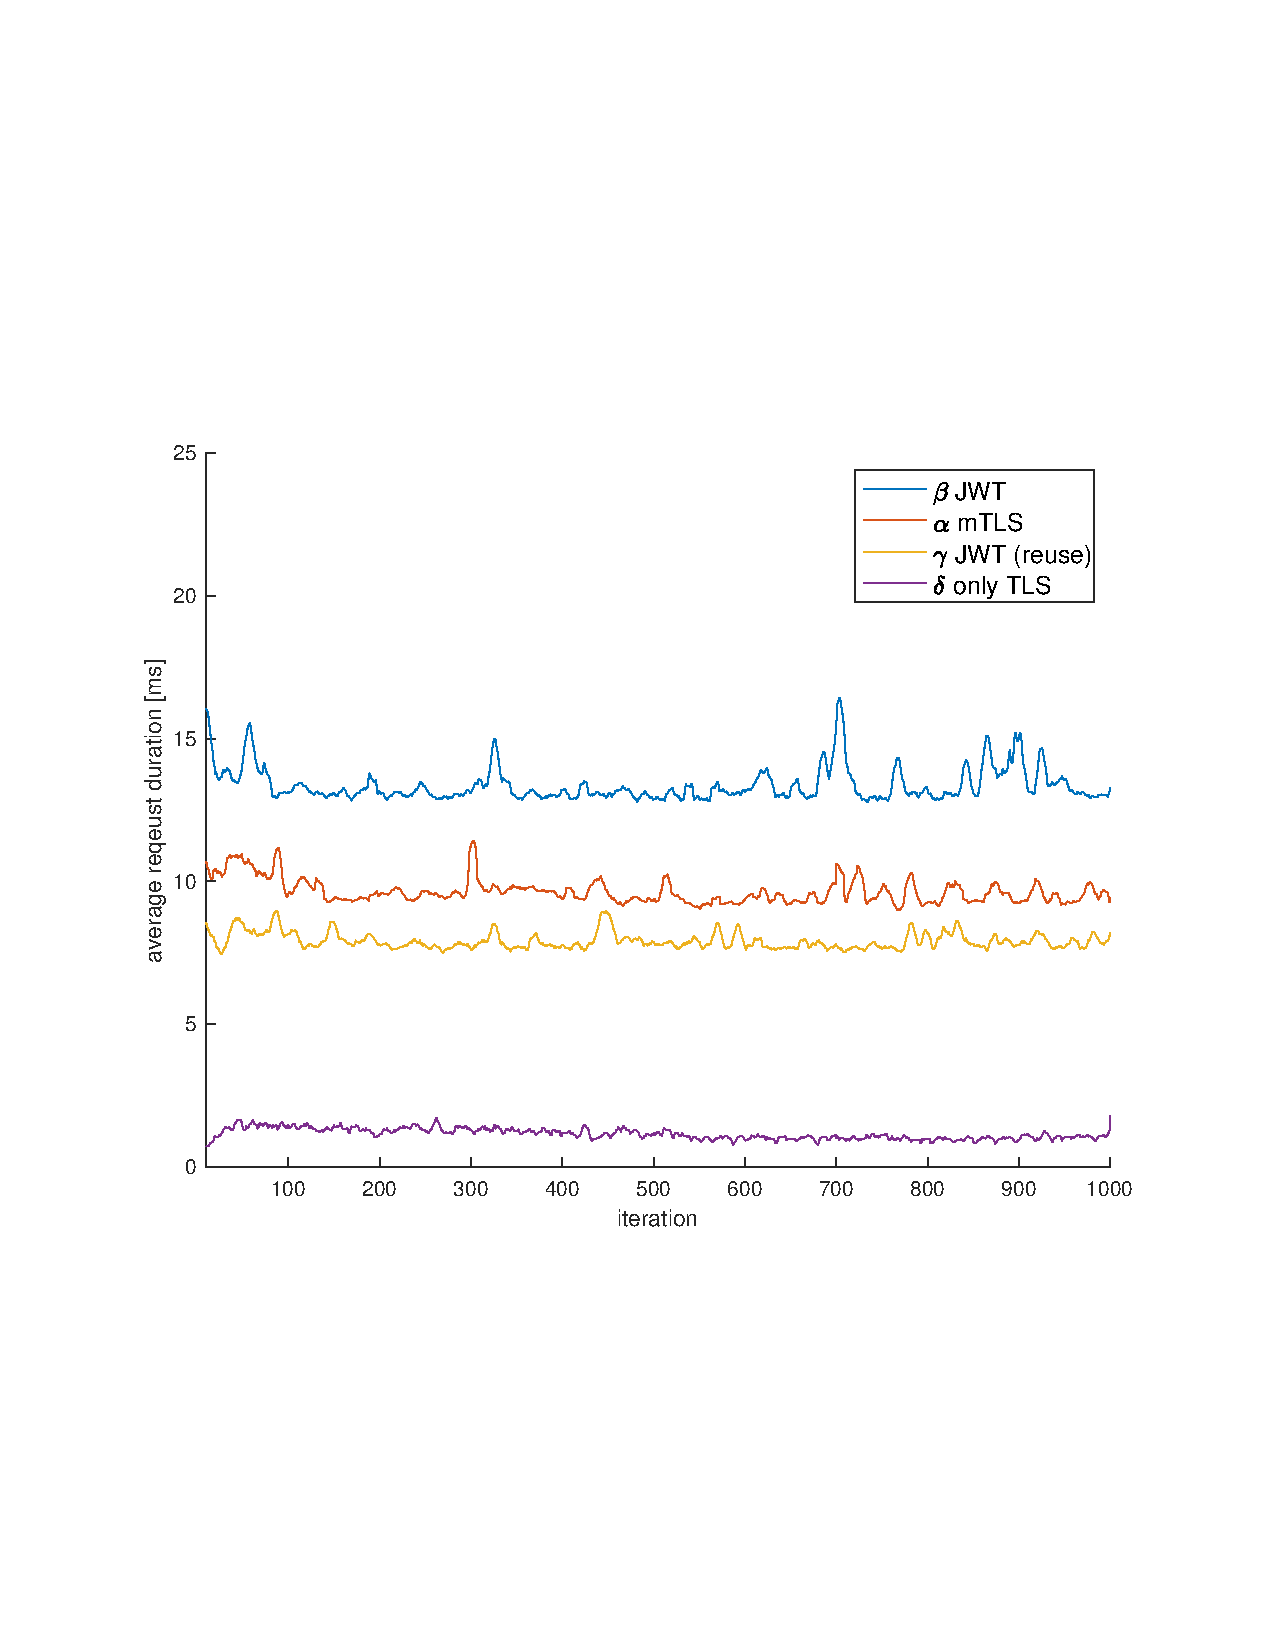
\includegraphics[trim=0 200 0 200, clip, width=\textwidth]{images/experiment/experiment-trend.pdf}
	\caption{Smoothened trend of the average request duration comparing the discussed authentication mechanisms excluding the first request}
	\label{fig:trend}
\end{figure}

\section{Conclusion}
This experiment compared the request durations of the two previously authentication mechanisms.
The results showed that the request durations between the mechanism using self-signed JWTs and mTLS are very similiar.
Depending on the implementation of the JWT approach it can consume up to 34\% more time or up to 20\% less time.
Therefore the performance is not the most crucial criterion when the two authentication mechanisms are compared since it's just a matter of milliseconds. 

Nevertheless for time critical projects in which each millisecond matters, self-signed JWTs are the better choice, since the performance can be optimized in multiple ways.
For example the certificates of the services can be distributed even before the first request is performed.
Or the validity timespan of the tokens can be increased so the same tokens can be used for a longer timespan.

\chapter{Final Remarks}
\label{cha:final_remarks}

\section{Discussion}
This thesis compared and explained the most popular mechanisms for mutual authentication in a microservice deployment.
Both mechanisms are based on public-key cryptography, but each mechanism has its own motivations and challenges.

Mutual TLS is an efficient and straightforward authentication mechanism.
The implementation of mTLS is very simple since the TLS protocol defines the processes.
Otherwise, mTLS does not provide many configuration parameters, and it does not allow to add custom functionalities, like sharing the user context without additional technologies.
Nevertheless, if a developer aims to implement only service-to-service authentication, mTLS is the preferred authentication mechanism.

As soon as nonrepudiation is required, self-signed JWTs are the superior authentication mechanism.
Furthermore, JWTs make identity propagation more convenient and allow the developers to customize the authentication mechanism and add additional parameters.
On the other hand, the implementation of self-signed JWTs is more challenging and requires each service to know how to work with JWTs.
Therefore choosing JWTs over mTLS would be unnecessary overhead when the target is implementing only service-to-service authentication.
The decision if the additional control of the approach using self-signed JWTs is worth the overhead has to be evaluated for each project independently.

The experiment of chapter~\ref{cha:experiment} showed that the performance of the compared authentication mechanisms is very similar.
According to the experiment results, the performance of the approach using self-signed JWTs is very dependent on the implementation of the mechanisms.
In some cases, using self-signed JWTs results in a lower request duration, but in some situations, it results in a higher request duration.
Therefore the performance is not a criterion that makes any mechanism superior to the other.

The biggest challenge of both authentication mechanisms is key management.
Both mechanisms require a PKI and require handling all associated key management tasks.
Therefore, implementing the authentication mechanisms is less challenging than the implementation of a key management system.
Nevertheless, the level of security that is provided using public-key cryptography is worth the expenses.

\section{Summary}
Service-to-service authentication is a requirement caused by the migration to the microservice architecture.
Function calls within the monolithic backend migrate to remote calls.
Remote calls have to assure authentication, confidentiality, and integrity.
Confidentiality and integrity can be assured using TLS, but authentication of both parties requires additional mechanisms.

This thesis compared two of the most popular authentication mechanisms for service-to-service authentication.
Therefore the fundamentals and concepts of the compared authentication mechanisms were described in detail.
Additionally, a project using the discussed mechanisms was reviewed, and the consequences of the different mechanisms were described.
In the end, an experiment comparing the performance of the discussed authentication mechanisms was performed, and the results were discussed.


%% Is just a file for the listings of the presentation, because the LaTeX template does not provide a simple way to include code
\chapter{Listings}

\begin{CsCode}
	...
	var userManagement = new UserMangagement();
	User user = userManagement.getUser(userId);
	...
\end{CsCode}

\begin{CsCode}
	...
	var userClient = new UserMangagementClient("http://usermanagement.swapindo.com/", Program.httpClient);
	User user = userClient.UserAsync(userId)
		.GetAwaiter()
		.GetResult();
	...
\end{CsCode}

%\chapter{Implementation}
\label{cha:Implementation}
This chapter shows an implementation of the authentication mechanisms discussed in chapter~\ref{cha:authentication_mechanisms}.
The trust the network approach is not implemented in this chapter because it is deprecated and should not be used anymore. 

This implementation aims not to teach how to implement the discussed authentication mechanisms. It should help to gain a good understanding of how the mechanisms work.
Security critical features like service-to-service authentication are not recommended to be implemented and maintained by developers, which are not specialized for software security.
Therefore it is always good to use software as a platform applications like Kubernetes.
The most popular service mesh for Kubernetes is Istio.
It provides all security mechanisms, which are implemented in this chapter.
The implementation of Istio might differ from the following implementation, but the concepts stay the same.

\section{Implementation of mTLS}
This chapter shows the implementation of service-to-service authentication using mutual TLS. 
The following snippets are based on an ASP.NET 5.0 Web API written in C\# and the keys are generated using the cli\footnote{Command line interface} of OpenSSL.
Even if the implementation looks different in other languages, the code snippets should help understand the used mechanisms in more detail.

\subsection{Create Certificate Authority}
The following commands will create a key pair and a certificate for the CA.
The parameters of the following commands might vary, depending on how security-critical an application is.
The certificate of the CA is self-signed and does only include the subject field.
The CA has a 4096-bit RSA key, which does not mean that a 2048-bit key is not valid, but a 4096-bit key is much harder to brute force.
The key pair is also encrypted using the AES algorithm with a 256-bit key. Therefore anybody who has physical access to the file also needs a password to read the content.
The certificate of the CA is valid for one year, this period always depends on the application.
\begin{enumerate}
    \item Create key pair: \\ 
    \lstinline{openssl genrsa -aes256 -passout pass:"capassword" -out ca.key 4096}
    \item Create self-signed certificate: \\
    \lstinline{openssl req -new -passin pass:"capassword" -key ca.key -x509 -days 365} \\
    \lstinline{-out ca.crt -subj "/CN=ca.swapindo.com"}
\end{enumerate}

\subsection{Create key pair and a signed certificate for a service} \label{sec:createkeypair}
The following commands will create a key pair and a certificate for a service. 
The CA signed the certificate and is later used in the TLS handshake.
Each service has to do this process, therefore it is good to use automation tools like Netflix uses Lemur~\cite{dias2020microservices}.
The certificates of the services get a shorter lifetime of 30 days, this might also differ depending on how security-critical the application is. 
Additionally, a PFX file is created, it is an encrypted container that includes both the certificate and the key pair.
The PFX file is not required, but it makes it more convenient to parse the file from a C\# program.
\begin{enumerate}
    \item Create key pair: \\ 
    \lstinline{openssl genrsa -aes256 -passout pass:"servicepassword" -out service.key 4096}
    \item Create certificate signing request: \\
    \lstinline{openssl req -passin pass:"servicepassword" -new -key service.key} \\
    \lstinline{-out service.csr -subj "/CN=adservice.swapindo.com"}
    \item Sign certificate, using the private key of the CA: \\
    \lstinline{openssl x509 -req -passin pass:"capassword" -days 30 -in service.csr -CA ca.crt} \\
    \lstinline{-CAkey ca.key -set_serial -01 -out service.crt}
    \item Create PFX file, which is later used, to send HTTPS Requests: \\
    \lstinline{openssl pkcs12 -export -out service.pfx -passin pass:"servicepassword" -inkey} \\ 
    \lstinline{service.key -in service.crt -passout pass:"passwordService"}
\end{enumerate}

\subsection{Certificate validation logic}
The code of listing~\ref{lst:CertificateAuthority} shows an implementation of the validation logic, implemented in a static class, the \textit{CertificateAuthority}.
The \textit{CertificateAuthority} makes use of the singleton pattern, which is good practice since the validations do not store any state, and the file which holds the CA certificate should not be parsed at each request.
The validation is done using an \textit{X509Chain} of the dotnet cryptography library.
The chain is configured to ignore revocation because the revocation is beyond the scope of this implementation.
Furthermore, the chain is configured to use the \textit{CustomTrustStore}, because this is the place where the appended certificates are stored.

The \textit{AppendCertificate} function is used to append the certificate of the self-signed root CA to the \textit{CustomTrustStore} of the chain.
The CA certificate could also be appended in the constructor of the CA, but providing a function for this purpose makes the class more flexible since multiple CAs can be added, and the path of the certificate can vary between the applications.

The validation of the certificate is performed in the \textit{ValidateCertificate} function. 
It uses the \textit{Build} function of the \textit{X509Chain}, which returns true or false, whether the certificate is valid or not.
Using the cryptographic functionalities of popular libraries is always safer than implementing them by hand.

\noindent \begin{minipage}{\linewidth}
\begin{CsCode}[label={lst:CertificateAuthority}, caption={CertificateAuthority class, that is responsible for the certificate validation~\cite{impsingleton,impvalidatecert,impx509chain}},captionpos=b]
 public class CertificateAuthority {
    private static X509Chain chain = null;
    private static CertificateAuthority instance = new CertificateAuthority();
    public static CertificateAuthority Instance { get { return instance; } }
    
    static CertificateAuthority() {
        // Create chain
        chain = new X509Chain();
        
        // Set options
        chain.ChainPolicy.RevocationMode = X509RevocationMode.NoCheck;
        chain.ChainPolicy.TrustMode = X509ChainTrustMode.CustomRootTrust;
    }
    
    public void AppendCertificate(X509Certificate cert) {
        // Add the certificate to the custom trust store
        chain.ChainPolicy.CustomTrustStore.Add(cert);
    }
    
    public bool Validate(X509Certificate2 cert) {
        try {
            return chain.Build(cert);
        } catch (Exception ex) {
            return false;
        }
    }
}
\end{CsCode}
\end{minipage}

\subsection{Service configuration}
The server, which hosts the application has to be configured to allow the client to send certificates. 
This process may vary, depending on the used technologies.
The code in listing~\ref{lst:ConfigureKestrel} shows how this is done using the Kestrel web server.
This only allows the clients to send certificates, but it does not validate them against the CA.
Therefore every request, which uses a valid certificate is considered valid, even if the certificate is signed by an unknown CA.

\noindent \begin{minipage}{\linewidth}
\begin{CsCode}[label={lst:ConfigureKestrel}, caption={Configure Kestrel to allow certificates~\cite{implkritnermtls}},captionpos=b]
webBuilder.ConfigureKestrel(kestrelOptions => {
    kestrelOptions.ConfigureHttpsDefaults(httpOptions => {
        httpOptions.ClientCertificateMode = ClientCertificateMode.AllowCertificate;
    });
});
\end{CsCode}
\end{minipage}

Listing~\ref{lst:ConfigureService} shows how the services are configured to verify that the incoming certificate is signed by the trusted root CA.
The validation is configured to neglect the revocation and allow only chained certificates. Otherwise, somebody could use the key pair of the CA itself to access the service.
If the certificate is considered valid, it is additionally checked by the \textit{CertificateAuthority}, which was shown in listing~\ref{lst:CertificateAuthority}.
If the client's certificate is valid and is signed by the CA, the client is authenticated and is allowed to access the functionalities of the service.

\noindent \begin{minipage}{\linewidth}
\begin{CsCode}[label={lst:ConfigureService}, caption={Configure the certificate authentication for the service~\cite{implkritnermtls}},captionpos=b]
services.AddAuthentication(CertificateAuthenticationDefaults.AuthenticationScheme)
.AddCertificate(options => {
    options.AllowedCertificateTypes = CertificateTypes.Chained;
    options.RevocationMode = X509RevocationMode.NoCheck;
    options.Events = new CertificateAuthenticationEvents() {
        OnCertificateValidated = context => {
            if (CertificateAuthority.Instance.Validate(context.ClientCertificate)) {
                context.Success();
            } else {
                context.Fail("Certificate validation failed");
            }
            return Task.CompletedTask;
        },
        OnAuthenticationFailed = context => {
            context.Fail("Certificate validation failed");
            return Task.CompletedTask;
        }
    };
});
\end{CsCode}
\end{minipage}

The code of listing~\ref{lst:ConfigureService} shows how to configure the client authentication for the service.
But the service has to be configured to use the implemented authentication mechanism.
Therefore the statement \lstinline{app.UseAuthentication();} has to be added to the \textit{Configure} function of the \textit{Startup} class. 
Since the service was configured to allow certificates and not to require them. 
The API functions can define whether a client needs a valid certificate or not.
This is done by appending the \lstinline{[Authorize]} annotation before the function declaration.
The code of listing~\ref{lst:ConfigureKestrel} can be adopted to require certificates, which would not allow any access to the API without a valid certificate.

\subsection{Use the certificate for requests}
Since the services consume the functionalities of other services, they have to be configured to use client certificates for their request.
The creation of a client certificate was shown in section~\ref{sec:createkeypair}.
Listing~\ref{lst:ConfigureHttpClient} shows how the client certificate is appended to a \textit{HttpClient}, which is later injected into the services, using dependency injection.
It is not required to use dependency injection for the HttpClient, but it is good practice to use it according to the documentation.
A considerable advantage of the dependency injection is that the pfx file does not have to be parsed for each request.
Instead, it is parsed once and injected into the controller when initialized.
The controller can then use the \textit{HttpClient} and perform requests without dealing with the client certificate.

\noindent \begin{minipage}{\linewidth}
\begin{CsCode}[label={lst:ConfigureHttpClient}, caption={Append Certificate to HttpClient~\cite{implclientfactory, implconfighandler}},captionpos=b]
services.AddHttpClient("mtlsclient")
.ConfigurePrimaryHttpMessageHandler(() => {
    HttpClientHandler handler = new HttpClientHandler();
    handler.ClientCertificates
        .Add(new X509Certificate2(@"service.pfx", "passwordService"));
    return handler;
});
\end{CsCode}
\end{minipage}

%Listing~\ref{lst:UseHttpClient} shows how the configured HttpClient is injected into a Controller and then used to perform a request.
%
%\noindent \begin{minipage}{\linewidth}
%\begin{CsCode}[label={lst:UseHttpClient}, caption={Use the injected HttpClient~\cite{impluseclient}},captionpos=b]
%[ApiController]
%public class ForwardUsersController : ControllerBase {
%    private HttpClient httpClient;
%
%    public ForwardUsersController(IHttpClientFactory factory) {
%        httpClient = factory.CreateClient("mtlsclient");
%    }
%
%    [HttpGet]
%    public async Task<string> Get() {
%        using (var response = await httpClient.GetAsync(apiUrl)) {
%            // process response
%        }
%    }
%}
%\end{CsCode}
%\end{minipage}

%%%-----------------------------------------------------------------------------
\appendix                                                             % Appendix 
%%%-----------------------------------------------------------------------------

%\chapter{Technical Details}
\label{app:TechnicalDetails}

%\section{JSON Web Token Registered Claims}
%\begin{table}[H]
%    \centering
%    \begin{tabular}{|l|l|p{7cm}|}
%    \hline
%        \textbf{Claim Identifier} & \textbf{Name} & \textbf{Content} \\
%    \hline
%        iss & Issuer & identifies the principle, that issued the JWT \\
%    \hline
%        sub & Subject & identifies the principle that is the subject of the JWT \\
%    \hline 
%        aud & Audience & identifies the principle that the JWT is intended for \\ 
%    \hline
%        exp & Expiration Time & identifies the expiration time on or after which the JWT must not be accepted for processing \\
%     \hline
%        nbf & Not Before & identifies the time before which the JWT must not be accepted for processing \\
%    \hline
%        ist & Issued At & identifies the time at which the JWT was issued \\
%    \hline
%        jti & JWT ID & provides a unique identifier for the JWT \\
%    \hline
%    \end{tabular}
%    \caption{JWT Registered Claims~\cite{jwtrfc}}
%    \label{tab:jwt_registered claims}
%\end{table}
 % Technical supplements

%%%-----------------------------------------------------------------------------
\backmatter                           % Back part (bibliography, glossary, etc.)
%%%-----------------------------------------------------------------------------

\MakeBibliography % References

%%%-----------------------------------------------------------------------------
% Special page for checking print size
%%%-----------------------------------------------------------------------------

%\chapter*{Check Final Print Size}

\begin{center}
{\Large --- Check final print size! ---}

\bigskip

\calibrationbox{100}{50} % width/height of box in mm

\bigskip

{\Large --- Remove this page after printing! ---}

\end{center}



%%%-----------------------------------------------------------------------------
\end{document}
%%%-----------------------------------------------------------------------------
